
\chapter{相关技术与工作}

\section{PortraitGen技术原理分析}

PortraitGen作为当前先进的肖像视频编辑技术,其核心创新点体现在以下三个关键方面。

\subsection{3D高斯场表示}

传统的视频编辑利用生成对抗网络(GAN)、去噪扩散模型等技术进行内容生成,但这些编辑技术
都无法保证视频帧之间的一致性;为了结果的连续性,许多工作提出了引入包括密集对应、帧间注意力
机制等方法,但由于缺乏对3D场景的理解与3D对象的先验认知,这些模型也没有办法保证视频的一致性。

\subsubsection{3D高斯场景表示}
在PortraitGen中,我们将视频编辑任务从2D提升至3D,并采用3D高斯溅射来表示场景。具体而言,
我们用数百万个3D高斯椭球来表示场景,对于每个以$\symbf{x}_0$为球心的高斯分布,我们有
\begin{equation}
    g(\symbf{x})=\exp{-\frac{1}{2}(\symbf{x}-\symbf{x}_0)^T\symbf{\Sigma}(\symbf{x}-\symbf{x}_0)}
\end{equation}
其中$\symbf{\Sigma}$为协方差矩阵,通过旋转和缩放控制椭球的形状,有分解
\begin{equation}
    \symbf{\Sigma}=\symbf{R}\symbf{\Lambda}\symbf{\Lambda}^T\symbf{R}^T
    \label{cov-decom}
\end{equation}
其中$\symbf{R}$为旋转矩阵,$\symbf{\Lambda}$为缩放矩阵。为了将三维的场景映射到二维平面,
我们还需要定义每个高斯椭球的不透明度$\alpha$和球谐函数,以控制光照和颜色信息。

\subsubsection{参数优化}
3D高斯场采用了可微分的溅射渲染,通过将3D高斯投影到2D屏幕空间,我们可以计算每个像素的颜色
\begin{equation}
    C(\symbf{p})=\sum_{i\in N}c_i\alpha_i\prod_{j=1}^{i-1}(1-\alpha_j)
\end{equation}
其中$c_i$为第$i$个高斯的颜色,基于视角可以由球谐函数决定。为了优化由稀疏点云重建的3D高斯场,
我们将给定视角下的渲染结果与真实结果进行比对,定义损失函数为
\begin{equation}
    \mathcal{L}=(1-\lambda)\mathcal{L}_1+\lambda\mathcal{L}_\text{D\_SSIM}
\end{equation}
其中$\mathcal{L}_1$为渲染的像素差异,描述了渲染结果与真是结果的光度差异;$\mathcal{L}_\text{D\_SSIM}$
为基于感知的损失函数,用于衡量图像的结构相似性。我们选用随机梯度下降(SGD)来优化3D高斯的参数,
包括高斯的位置、协方差、不透明度和颜色。注意到协方差矩阵$\symbf{\Sigma}$有其物理意义,只有半正定矩阵
是合理的,但是SGD优化难以添加约束条件,因此考虑到协方差矩阵的分解形式~\eqref{cov-decom},我们转而对
代表缩放的向量$\symbf{s}$与代表旋转的四元数$\symbf{q}$进行优化。

初始的高斯球直接由点云重建,而这种2D到3D的映射往往无法满足精细表示的需要,因此我们的优化也需要
有3D高斯的自适应操作,包括:
\begin{enumerate}
    \item \textbf{删除}:当高斯球的透明度小于阈值$\epsilon_{\alpha}$时,说明此时高斯球对场景表示的贡献较小,可以删除;
    \item \textbf{密集}:区域没有被高斯球覆盖与过度覆盖都说明当前重建不够,需要修改目前的高斯球,以更好地表示场景:
        \begin{itemize}
            \item 当区域没有被高斯球完全覆盖时,将已有的高斯球复制并按照梯度方向移动到空白位置;
            \item 当区域被高斯球过度覆盖时,将大高斯球按照$\phi=1.6$的比例分成两个小的高斯球;
        \end{itemize}
    \item \textbf{特殊处理}:与其他体积表征的方法类似,在相机附近可能有悬浮高斯球导致优化停滞,因此需要每迭代3000轮后将这些高斯球的透明度$\alpha$设置为接近0。
\end{enumerate}

\begin{figure}[ht]
    \centering
    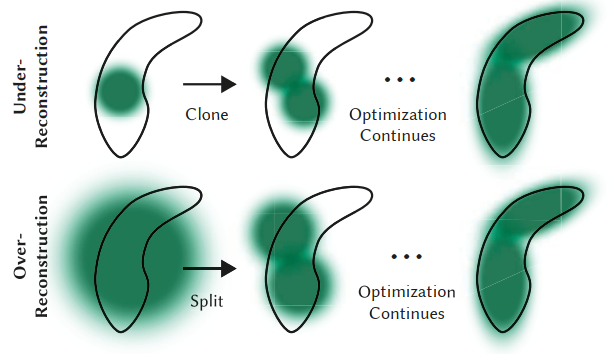
\includegraphics[width=0.5\textwidth]{source/img/gauss_recon.png}
    \bicaption{高斯球的密集}{Densification of Gaussian}
\end{figure}

\subsubsection{可微光栅化渲染}

3D高斯的光栅化过程主要分为四个步骤:
\begin{enumerate}
    \item \textbf{分块}:将屏幕空间划分为$16\times 16$的小块,对每个小块保留与视锥相交超过99\%的高斯球;
    \item \textbf{排序}:为每个高斯分配一个键,携带视图空间深度与块ID信息,并利用GPU基数排序,为每个块生成一个高斯列表;
    \item \textbf{光栅化}:每个块启动一个线程块,协作加载高斯到共享内存。对每个像素,从前到后遍历列表,累积颜色和$\alpha$值,当像素的$\alpha$值达到饱和(接近1)时,停止处理;
    \item \textbf{反向传播}:在反向传播时,重新遍历排序后的高斯列表,但方向是从后到前。这样可以在计算梯度时恢复中间的$\alpha$值,无需存储中间结果增加内存消耗。
\end{enumerate}

\subsection{神经高斯纹理机制}

在标准的3D高斯溅射中,每个高斯球的颜色通过球谐函数的系数来表示,而这种表示存在一些问题:一方面,球谐系数仅能建模低频的光照变化,难以表现高频的细节,如笔触、艺术风格等;另一方面,
强制使所有视角严格遵守物理光照,阻碍了3D高斯在会真实感渲染方面的应用,例如卡通风格的轮廓线等。portraitgen用可学习的特征来代替每个3D高斯的球谐函数,实现了更强的表达能力。

我们使用SMPL-X作为人体模型的表示方法,SMPL-X的定义为
\begin{align}
    M(\beta,\theta,\psi)&=W(T_p(\beta,\theta,\psi), J(\beta),\theta, \mathcal{W})\\
    T_p(\beta,\theta,\psi)&=\bar{T}+B_S(\beta;\mathcal{S})+B_E(\psi;\mathcal{E})+B_P(\theta;\mathcal{P})
\end{align}
其中$\beta$、$\theta$、$\psi$分别为形状、姿态与表情参数;$W$为线性混合蒙皮函数,$J$为稀疏线性回归器,可以从输入网格顶点回归出三维关节位置,$\mathcal{W}$
为混合权重,在旋转时起平滑作用。

我们在SMPL-X模型的UV表面绑定3D高斯场$\phi$,通过纹理坐标$(u,v)$来索引特征,这样在网格动态变形时高斯能随之运动从而保持拓扑的一致性。利用UV空间的参数映射$\mathcal{G}$,我们可以得到某一帧的3D高斯场
\begin{equation}
    (\symbf{X}_0,Q,S,O,F)=\mathcal{F}(M(\beta,\theta,\psi),\mathcal{G},\phi)
\end{equation}

\subsection{表情相似性引导与感知编辑}

在portraitgen的编辑过程中,需要迭代编辑视频数据集,而在反复编辑视频帧的过程中,每次编辑都可能引入微小表情偏差,多次迭代后偏差放大,
导致面部表情和个性化特征会逐渐退化,如笑容僵硬、五官变形等。为了解决这一问题,我们采用3D表情识别模型EMOCA提取表情潜码
\begin{equation}
    z_{\text{exp}}=E_{\text{EMOCA}}(I) \in \mathbb{R} ^{50}
\end{equation}
并通过$L2$损失约束编辑后的表情特征
\begin{equation}
    \mathcal{L}_{\text{exp}}=||E_{\text{EMOCA}}(I_{\text{edit}})-E_{\text{EMOCA}}(I_{\text{src}})||_2^2
\end{equation}
实现了仅约束表情肌肉运动而不限制外观风格变化。

